\documentclass{article}
\usepackage{iclr2026_conference,times}

\input{math_commands.tex}

\usepackage{xcolor}
\newcommand{\red}[1]{\textcolor{red}{#1}}
\newcommand{\todo}[1]{\textcolor{magenta}{\textbf{[TODO: #1]}}}

\usepackage{amsmath,amssymb,amsthm}
\usepackage{booktabs}
\usepackage{graphicx}
\usepackage{tikz}
\usetikzlibrary{arrows.meta,positioning,calc,fit,backgrounds}
\pagestyle{empty}
\definecolor{inputgray}{RGB}{76,84,92}
\definecolor{predblue}{RGB}{42,104,145}
\definecolor{predgreen}{RGB}{42,124,91}
\definecolor{controlred}{RGB}{181,74,58}
\definecolor{controlorange}{RGB}{196,116,42}
\definecolor{fitpurple}{RGB}{102,75,145}

\usepackage{adjustbox}
\usepackage{algorithm}
\usepackage{cancel}
\usepackage{url}
\usepackage{hyperref}


% \newcommand{\Sigma}{\mathbf{\Sigma}}
% \newcommand{\R}{\mathbb{R}}
% \title{When Test Error Hides Directional Failure: Random Matrix Theory for Accentuation in Ridge Regression}
% \title{Why a good predictor can be a bad controller: \\A Random Matrix Analysis for Dissociation of Neural Prediction and Control}
\title{When Good Brain Predictors Make Bad Brain Controllers: A Regression Theory of Prediction–Control Dissociation}

% Keep anonymous for ICLR submission.
\author{Anonymous Authors}

% Compatibility layer for theorem environments imported from LyX.
% Define localized names before amsthm binds them to environment headings.
\providecommand{\theoremname}{Theorem}
\providecommand{\propositionname}{Proposition}
\providecommand{\lemmaname}{Lemma}
\providecommand{\corollaryname}{Corollary}
\providecommand{\examplename}{Example}
\providecommand{\remarkname}{Remark}

\theoremstyle{plain}
\newtheorem{thm}{\theoremname}
\newtheorem{theorem}[thm]{\theoremname}
\newtheorem{proposition}[thm]{\propositionname}
\newtheorem{prop}[thm]{\propositionname}
\newtheorem{lemma}[thm]{\lemmaname}
\newtheorem{lem}[thm]{\lemmaname}
\newtheorem{corollary}[thm]{\corollaryname}
\newtheorem{cor}[thm]{\corollaryname}
\theoremstyle{definition}
\newtheorem{example}[thm]{\examplename}
\theoremstyle{remark}
\newtheorem{remark}{\remarkname}



%\iclrfinalcopy
\begin{document}
\maketitle

\begin{abstract}
% Modern learning systems are often evaluated by average in-distribution error, yet scientific and perceptual applications frequently probe a learned model along a distinguished direction: a response axis, a feature vector, or an intervention path. We study this mismatch in a solvable high-dimensional setting. For ridge regression with anisotropic Gaussian covariates, we derive deterministic equivalents for the per-eigenmode coefficient error and for an \emph{accentuation} error obtained by moving along the learned direction rather than the ground-truth direction. The theory decomposes coefficient error into three interpretable terms: regularization bias, finite-sample signal fluctuation, and finite-sample noise amplification. It predicts when average generalization and accentuation error disagree, and yields a crossing criterion for the noise level at which the dominant failure mode changes. Monte Carlo experiments across isotropic, power-law, and natural-image spectra validate the formula up to dimension $10{,}000$. The analysis identifies a second-order limitation of leading deterministic equivalents: the mean alignment is accurately predicted, while the variance of the alignment ratio dominates accentuation error in high-noise regimes. These results give a minimal theory for directional failure modes that are invisible to scalar test error.
% In visual neuroscience, many people have found there are many models
% that could predict neurons well on held out data but cannot generate
% perturbations to control them. Further, the control success is more
% predicted by structure of input gradient instead of metrics about
% the representation geometry.
% Here we show that these phenomena can be captured by linear model.
% The key idea is failure of control is a special kind of OOD generalization
% failure, where the distribution is model-generated. This self-generated
% distribution induced interesting structure in the evaluation metrics
% (R2, slope, MSE) on it, different from the classic generalization
% error.
% In Ridge regression, we derived the leading order (deterministic equivalent)
% approximation for the generalization error and control error, showing
% their differences. We show that the failure in control can still happen
% for noisy regression on non-isotropic data, even when the regularization
% parameter is selected via cross validation.
% Extending the analysis to linear feature regression case, we show
% that the generalization error and control error has different summary
% statistics -- generalization error cares about feature space covariance
% while control cares about the feature outer product themselves.
% We specifically characterized the \textit{gauge invariance
% group} of the feature map, which will not change the
% classic generalization error and CV selection; but changes the control
% / accentuation error dramatically.
% This shows our thesis that even for linear feature regression, prediction
% and control can be dissociated, and inspire us to look deeper into
% the gradient structure of feature maps.
Models that predict visual-neuron responses similarly well on held-out images can differ sharply in the stimuli they generate and in their ability to control those neurons. Experimental control success also tracks the structure of a model’s input gradient more closely than conventional measures of predictive performance. We study this prediction–control dissociation in a linear teacher–student model. Ordinary generalization evaluates a fitted predictor on the natural-image distribution; feature accentuation instead evaluates it on a distribution generated along its own fitted direction. This change of distribution gives accentuation error, \(R^2\), and response slope a different dependence on estimation error than standard test loss. Using deterministic equivalents for ridge regression, we show that prediction-optimal regularization generally differs from control-optimal regularization: cross-validation for prediction can therefore leave substantial control error under noisy, anisotropic data. We then extend the analysis to fixed linear feature maps. Prediction depends on the feature covariance and its alignment with the teacher, whereas control additionally depends on the feature map’s Euclidean geometry. We construct a family of feature maps that preserves leading-order generalization error and its cross-validated optimum while changing accentuation performance. These results identify input-gradient geometry as a diagnostic of control failure that predictive accuracy alone cannot provide.
\end{abstract}

\section{Introduction}
One dream in the neuroscience is to build a "digital twin" of the real brain which predicts the activity of the brain, then we can leverage it for control, i.e. drive the brain to the target state.
Previous works have showed success in control neural activities in model free and model based fashion.
In model free fashion, ...
In model based fashion, an explicit predictive model of neural activity was built, and then the researcher "plan" against the predictive model, and create stimuli that drive the system to a target state.

One simplest version is instantiated in the recent study by Prince, Wang et al.
One striking finding is that even though many models are basically equally good at predict the brain, they are not as effective in control or modulate the brain.

% Recent works show that despite similar prediction accuracy on held out samples, the models have dramatically different performance in controlling the neurons and proposing the samples.
This finding itself is a bit puzzling.
In this work, we gave a unified account for these phenomena using a simple linear regression.
We show that the same dissociation can exist even in linear models.
In a certain sense, the failure of control can be interpreted as failure of "out-of-distribution" (OOD) prediction, and specifically in a case where the evaluation distribution is self-generated.
We precisely characterized the scaling of accentuation and held-out prediction error and how that depends on noise, spectral structure, feature space and other properties of the learning problem.

\begin{figure}
    \centering
    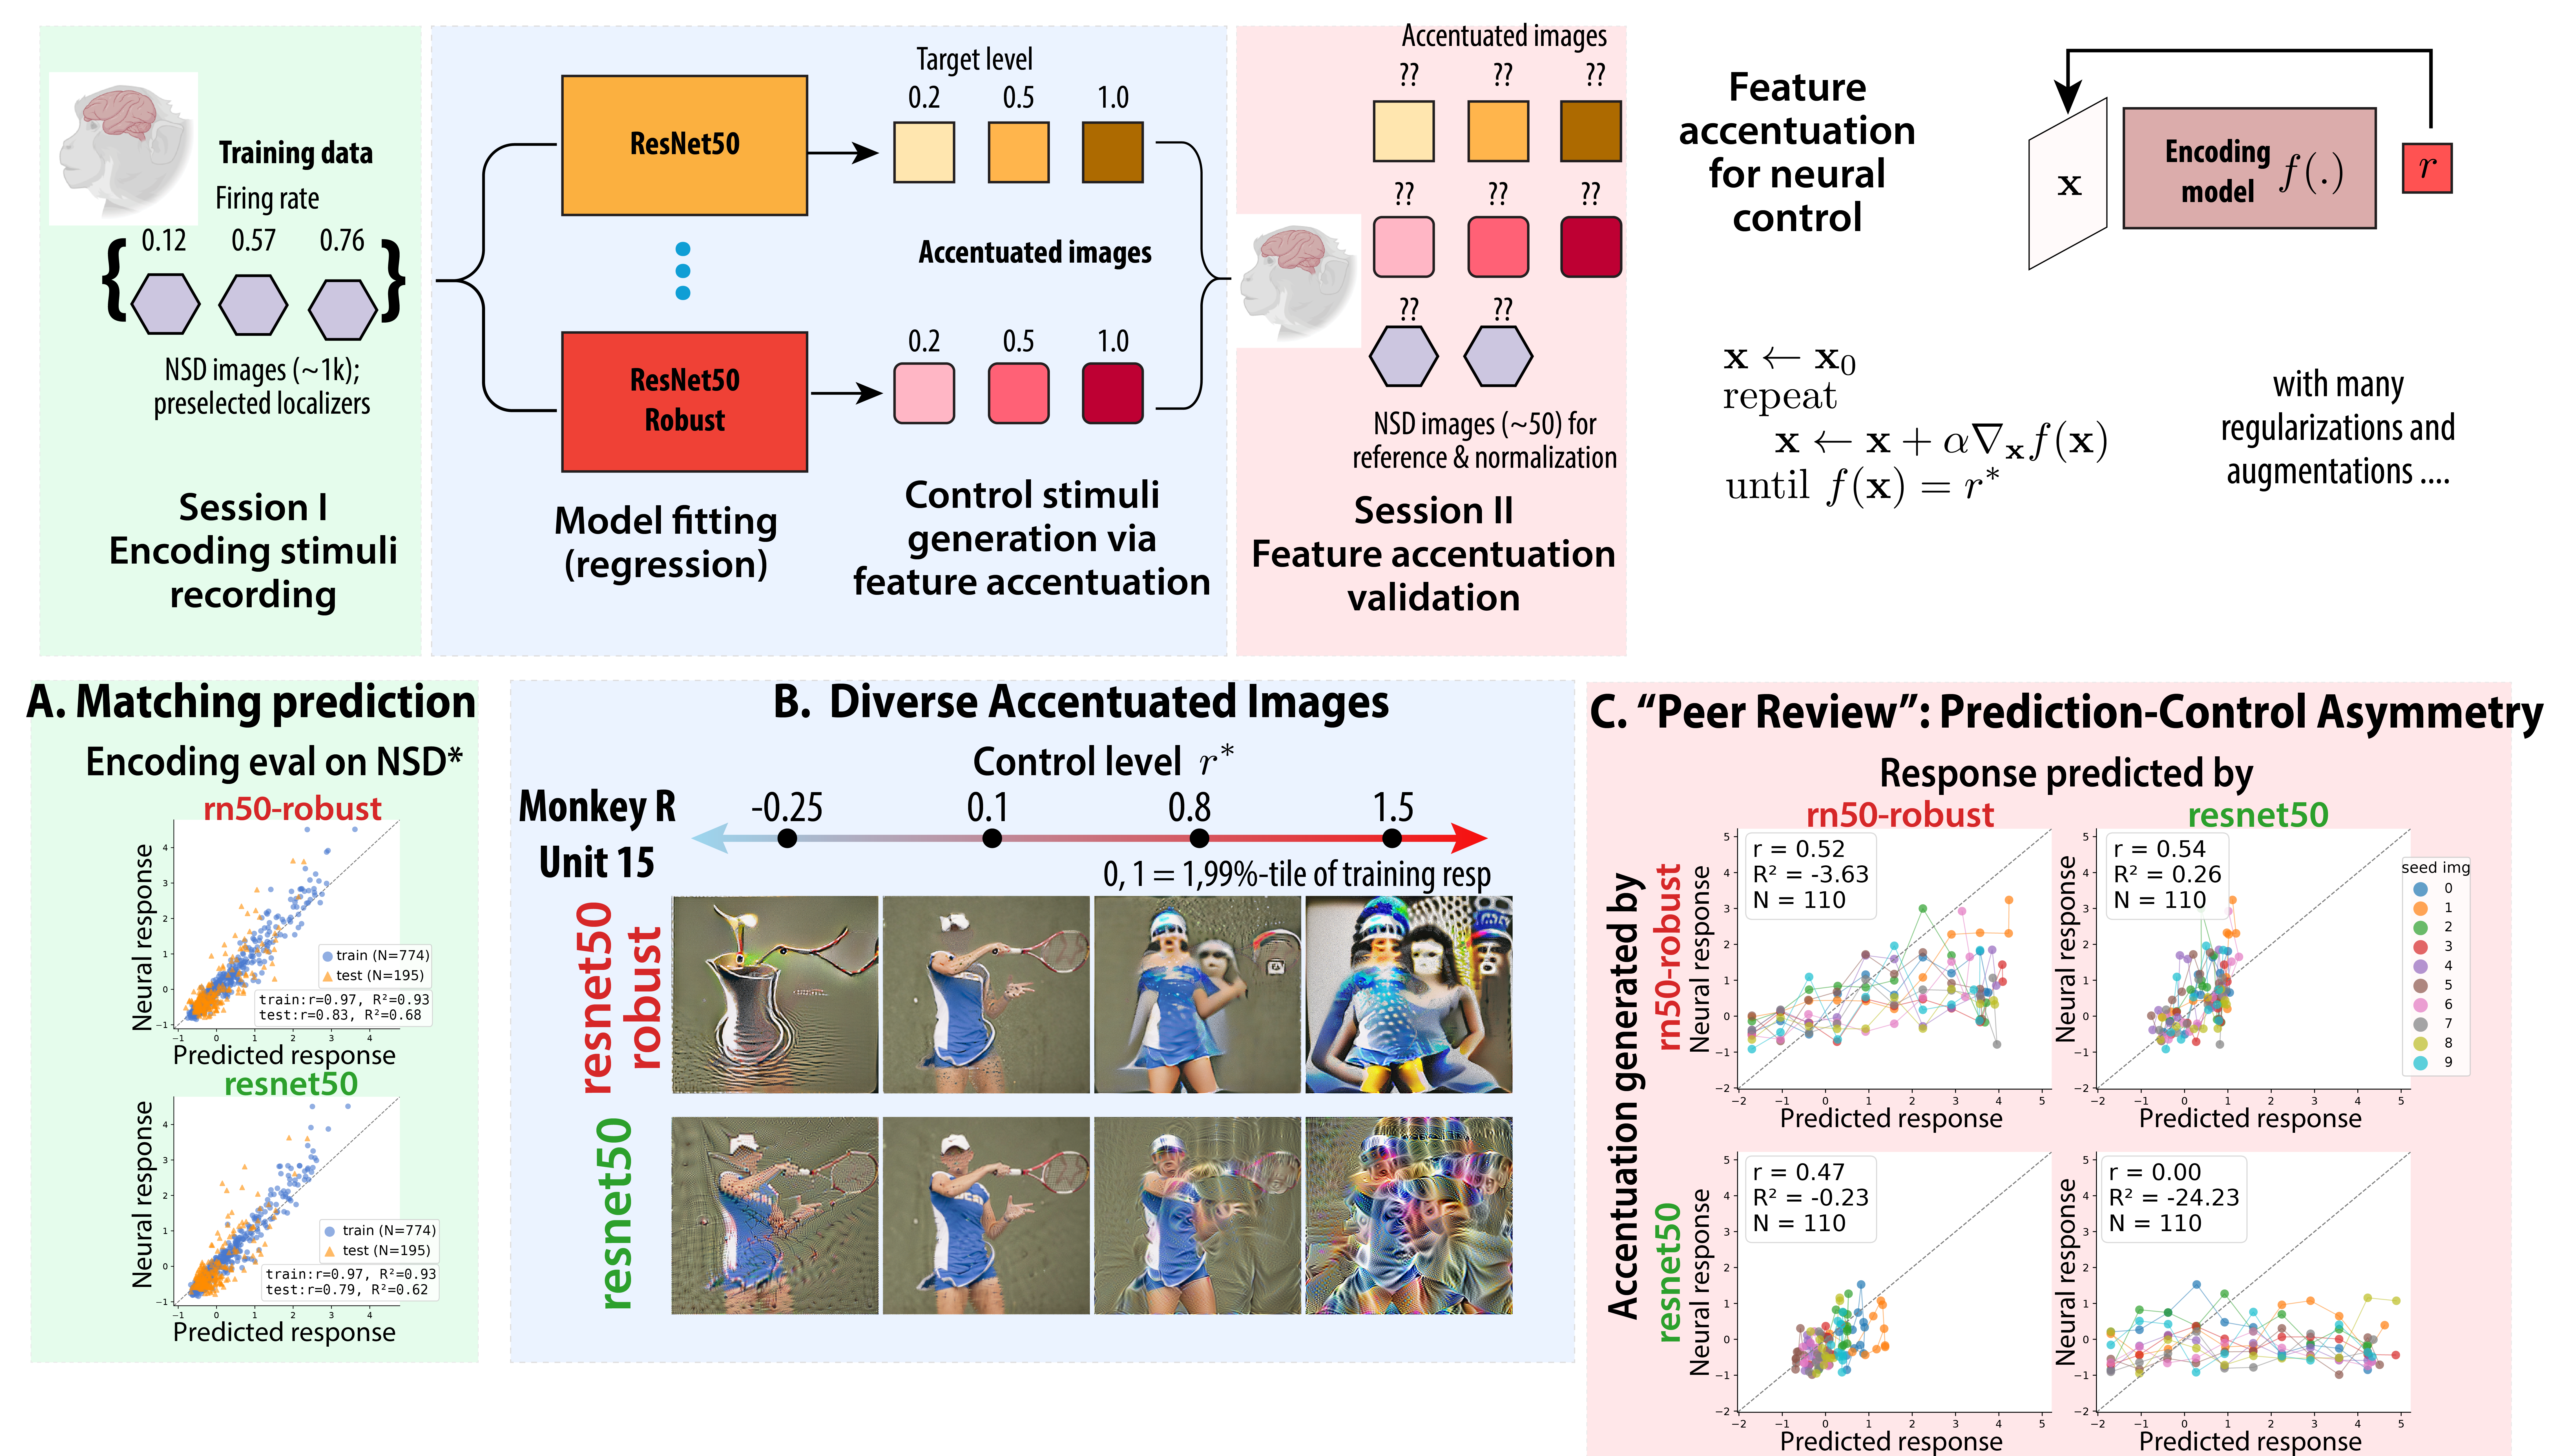
\includegraphics[width=\linewidth]{figures/Figure_NeuroCtrl_results.png}
    \caption{\red{\textbf{Motivating neuronal-control results.} Top: fitted encoding models generate images targeting graded neural responses, which are then tested in vivo. \textbf{A:} ResNet50 and ResNet50-Robust predict held-out natural-image responses similarly. \textbf{B:} The same seed and response targets yield visibly different accentuations. \textbf{C:} Cross-evaluation of the two stimulus sets illustrates the distinction between generating a useful sweep and tracking the neural responses to another model's sweep.}}
    \label{fig:Setup_NeuroControl_Results}
\end{figure}

\section{Key phenomena from neuronal control experiments}
We summarize and reproduce the results from the data of the closed-loop experiments of \citet{prince2026parametric}, which motivate the distinction between prediction and control (Fig.~\ref{fig:Setup_NeuroControl_Results}). 

\paragraph{Experimental setup.}
The experiments have four phases (Fig.~\ref{fig:Setup_NeuroControl_Results} A): 
\textbf{I.} First, visual cortical neuronal responses to a fixed set (\~1000) of natural image stimuli (mixture of Natural Scene Dataset shared images, and segmented objects) during fixation were recorded (using arrays and neuropixels). 
\textbf{II.} Next, encoding models are fitted: linear regressing neuronal responses onto the top PCA of the features in 10 DNN backbones (Tab.~\ref{}), with optimal Ridge regularization and layer selected via cross validation. These neuronal predictive models are denoted $f(.)$. 
\textbf{III.} Then, control (\textit{"accentuated"}) stimuli were generated: initialized from 10 seed images $\x_0$ selected from NSD, one perform \textit{feature accentuation} on each model $f_i$, roughly iterating $\x\gets \x +\nabla_{\x}f(\x)$, until $f(\x)$ reaches a target level $y^*$. In practice, preconditioning of the gradient and augmentation during optimization was done \citep{hamblin2024feature}, so more robust optima are found. For each seed, one select $11$ $y^*$ levels with uniform spacing, spanning the natural dynamic range of the neuron (range over training set), resulting in $1100$ accentuated images per target neuron. 
\textbf{IV.} Finally, one tested these images (along with some held out natural images) in the next recording session, 
recording actual neuronal responses of the same sites to these images -- designed by the 10 models to linearly modulate the neuronal firing. 
The premise is that, if the predictive model $f$ is a faithful model of the neuron, the designed stimuli should be able to control the neuronal firing with \textit{model predictive control}. So the difference between the 10 models signify their difference in \textit{control capability}, while the prediction accuracy on the the held out natural images shows the \textit{prediction capability}. 
This procedure is replicated for $25$ visual cortical sites in 5 primates, spanning V2,V3,V4,aIT,pIT,STS. Figures were reproduced using the published data. 


\paragraph{Similar held-out prediction, divergent control.}
\red{The nine trained models were tightly matched on natural-image re-test responses (model-mean Pearson $r=0.58$--$0.61$), yet their ability to predict and modulate responses to their own accentuated stimuli diverged sharply. Across all ten models, mean control correlation fell to $r=0.45$, with substantially greater between-model spread than on natural images. Many models generated conspicuous texture or high-frequency changes while achieving the requested \emph{model-predicted} response, but the measured neural response was weaker. In one reported site, natural-image re-test prediction reached $r=0.81$ whereas the accentuation control slope was only $0.05$ (a slope of $1$ would indicate calibrated control).}

\paragraph{Asymmetry of recognition and generation.}
When a model fails to \textit{generate} images and control neurons, could it \textit{recognize} the success of other models' control?
In the so-called \textit{peer-review} analysis, we send the accentuation images generated by A model to B model, and evaluate the B model's neural prediction accuracy on A models' generation. One can see ResNet50-robust (\texttt{robust})'s generation modulate neuronal firing as predicted; while neurons are almost not modulated by ResNet50 (\texttt{RN50})'s generation (Fig.~\ref{fig:Setup_NeuroControl_Results}C diagonal panels), showing the much stronger control capability of \texttt{robust}, while both overestimated the magnitude of their modulation. 
However, when showing generated images from strong controller (\texttt{robust}) to the weaker controller (\texttt{RN50}), the Pearson r is also good, with a more calibrated magnitude, and much less worse R2. 
Similarly, in the inverse direction, the stronger controller can also predict the neuronal responses on generated images from the weaker controllers. 
This create an interesting "assymmetry", models can recognize good successful control images, but cannot generate good controlling images themselves. 
The structure of peer review matrix between the 10 models are showed in App.~\ref{???}.
\iffalse
\red{The illustrative cross-evaluation in Fig.~\ref{fig:Setup_NeuroControl_Results}C separates evaluating a stimulus from generating it. For the shown site, ResNet50-Robust's images produced graded neural responses that both it and ordinary ResNet50 could track (response correlations $r=0.52$ and $0.54$, respectively). Ordinary ResNet50's own images, by contrast, barely modulated the neuron despite large predicted changes (self-evaluation $r\approx0$, $R^2=-24.23$). Here ``recognition'' means tracking response ordering, not calibrated amplitude: even the robust model's own $R^2$ is negative. This is a selected example, not a population estimate.}
\fi 

\paragraph{Control tracks input-gradient structure.}
What predicts the success of neuronal control? Apparently, the top-2 most performant neuronal control models are both adversarially trained or finetuned \cite{advers}. 
Generally, if one quantify the structure of the input gradient $\nabla_{\x} f$, one can see the stronger control models have perceptually better gradient: the gradient has more Fourier power in the low frequency band, and the spectral profile shows more natural image like fall off. This fall-off exponent (or some related spectral concentration measures) the can predict the control success across the $250$ model x neuron pairs \red{(site-level $r\approx0.65$; model-mean $r=0.91$). The association persisted after excluding the two adversarially trained models (site-level $r=0.26$), whereas the relationship with adversarial sensitivity did not.}
\iffalse
\red{Across the $250$ site--model encoding axes, low-frequency concentration of the input gradient predicted control slope (site-level $r\approx0.65$; model-mean $r=0.91$). The association persisted after excluding the two adversarially trained models (site-level $r=0.26$), whereas the relationship with adversarial sensitivity did not. Thus the observed failure is linked to \emph{which input directions} a model uses to change its prediction, not simply to how well it predicts natural images. Our linear theory isolates a tractable version of this directional mismatch; it does not claim that the DNN gradients or neuronal responses are globally linear.}
\fi

\begin{figure}[!htp]
    \centering
    \includegraphics[width=\linewidth]{figures/Figure_LinearToyModel.png}
    \caption{\textbf{A linear model recapitulating the phenomena}
    \textbf{Geometry of prediction--accentuation dissociation.}
    Natural-distribution prediction suppresses errors along low-variance directions through the covariance metric $\Sigma$; Accentuation instead evaluates the model on a path selected by the student weight itself (right), so a component that is nearly invisible in distribution can dominate control.}
    \label{fig:linear-dissociation-geometry}
    \label{fig:LinearToyExample_Geometry}
\end{figure}
\section{A random matrix characterization of the dissociation}
\label{sec:linear-rmt}

\red{We first define how generalization, accentuation, and peer review evaluate the same fitted weight under different distributions. We then use a two-dimensional example to expose the geometry of their dissociation, before asking how finite-sample ridge regression produces the relevant weight errors. In the geometric example the student weights are chosen directly; from Sec.~\ref{sec:pixel-ridge} onward, they are generated by learning from noisy data.}
\red{Our aim is to isolate three ingredients that create the dissociation already in a linear model: an anisotropic input spectrum, finite-sample learning from noisy targets, and the geometry of the feature map.}

Here we consider a classical set up where a linear model is learning from a linear teacher with additive noise \citep{dobriban2018high,hastie2022surprises}. % This system is very well studied, with ample beautiful papers.

\subsection{Set up: Linear noisy teacher student and feature accentuation}
\label{sec:linear-setup}
% \subsection{Teacher Student setup and different evaluations of the same predictor}

\paragraph{Teacher-Student}
We assume inputs $\x\in\mathbb{R}^d$ are drawn from $\mathcal{N}(0,\Sigma)$. The teacher has weight $\bstar\in\mathbb{R}^d$, and the observed response contains additive Gaussian noise $\epsilon\sim\mathcal{N}(0,1)$ at level $\sigma$:\todo{see if Gaussian data assumption can be lifted}
\[
y=\x^{\top}\bstar+\sigma\epsilon
\]
The student model is bias-free linear model with weight $\bhat$,
which we will extend to effective weights in linear feature case in Sec.~\ref{sec:feature-ridge}.
\[
f(\x)=\x^{\top}\bhat
\]
The student observes $n$ training pairs $\{\x_i,y_i\}_{i=1}^n$. We stack the inputs into $X\in\mathbb{R}^{n\times d}$, the responses into $\mathbf y\in\mathbb{R}^n$, and the realized noise into $\eta\in\mathbb{R}^n$, so that $\mathbf y=X\bstar+\sigma\eta$ and $\hat\Sigma=X^\top X/n$.

\paragraph{Evaluation}
For classic held-out prediction, we sample fresh samples from the population data distribution, and evaluate on it, thus the evaluation distribution is $\mathcal{N}(0,\Sigma)$ and the classic generalization error reads %can be written as
\begin{equation}
    E_{gen}=\mathbb{E}_{\x\sim \mathcal{N}(0,\Sigma)}[\|f(\x)-\x^\top\bstar\|^2]=(\bhat-\bstar)^\top\Sigma(\bhat-\bstar)
    \label{eq:gen-risk}
\end{equation}
\red{Eq.~\ref{eq:gen-risk} is the population risk conditional on the fitted weight $\bhat$. Below, $E_{gen,DE}$ denotes its deterministic equivalent after the training-data and response-noise fluctuations concentrate.}
For accentuation and control, however, the student proposes modified inputs based on its own weight.
Starting from a seed $\x_0$, gradient-based optimization of $f_{\bhat}(\x)=\x^\top\bhat$ moves along $\nabla_{\x}f_{\bhat}=\bhat$.
The solution of gradient descent i.e. the minimum-norm change that reaches the student-predicted target $y^*$ is
\begin{equation}
    \x_{acc}(y^*)
    =\x_0+\frac{y^*-\x_0^\top\bhat}{\|\bhat\|^2}\bhat.
    \label{eq:linear-accentuation-path}
\end{equation}
Thus the fitted weight is not only a predictor: it also determines the distribution i.e. direction along which the predictor is evaluated $\x_{0}+\alpha\bhat,\alpha\sim p(\alpha)$.
\footnote{This is an idealized version of deep-network feature accentuation, which may additionally use gradient preconditioning, augmentation, and image priors.\cite{hamblin2024feature,Fel_maco} }
% and then the model prediction is evaluated on it.
In the main paper, we assume a single seed image, $\x_{0}=0$,
and $\alpha$ is sampled from a centered distribution ($\mathbb{E}[\alpha]=0$) which makes the \emph{predicted model variance} match with the natural variance of teacher, e.g.
\begin{equation}
\mathrm{Var}[\alpha]({\bhat}^{\top}\bhat)^2={\bstar}^{\top}\Sigma\bstar
\label{eq:variance-matching}
\end{equation}
In \red{Appendix~\ref{sec:app-evaluation-distributions}}, we discuss the extension to non-centered seed images and multiple seed images.
As a result, the model is evaluated on the self-generated rank-1 distribution
% \[
% \x_{0}+\alpha\bhat.
% \]
\begin{equation}
    E_{acc}=\mathbb{E}_{\x=\x_{0}+\alpha\bhat;\alpha\sim p(\alpha)}[\|f(\x)-\x^\top\bstar\|^2]=\mathrm{Var}[\alpha]\big({\bhat}^{\top}(\bhat-\bstar)\big)^{2}
    \label{eq:accentuation-path-error}
\end{equation}
For peer review, model is evaluated on the accentuation path created
by other models with weight $\bprime$, with similar structure
% \[
% \x_{0}+\alpha\bprime
% \]
\begin{equation}
    E_{peer}=\mathbb{E}_{\x=\x_{0}+\alpha\bprime;\alpha\sim p(\alpha)}[\|f(\x)-\x^\top\bstar\|^2]=\mathrm{Var}[\alpha]\big({\bprime}^{\top}(\bhat-\bstar)\big)^{2}
    \label{eq:peer-path-error}
\end{equation}
Structurally, generalization error evaluate the teacher student deviation $\bhat-\bstar$ weighted over the full natural data covariance $\Sigma$, while accentuation focused on one direction selected by the student $\bhat$, and peer-review focus on one direction selected by the peer $\bprime$. One can easily see this introduces an out-of-distribution generalization problem. 


\subsection{Structure of the generalization and accentuation error}
\label{sec:evaluation-metrics}
% Using the Lemma \ref{lem:pred_error}\ref{lem:R2_pred_obs}\ref{lem:Pearson-r_pred_obs}\ref{lem:linear_slope},
% we can write down various form of evaluation metrics, MSE, R2, slope,
% Pearson r, given the mean and covariance $\mu_p,\Sigma_p$ of the evaluation distributions.

The key difference between classic generalization, accentuation and peer
review error can be seen via the (mean and) covariance of their evaluation
distribution ($\mu_p,\Sigma_p$). We can write down the form of MSE, R2, slope,
Pearson r in the the following Table \ref{tab:evaluation-metrics}, using Lemma \ref{lem:pred_error},\ref{lem:R2_pred_obs},\ref{lem:Pearson-r_pred_obs},\ref{lem:linear_slope}. 
We note that Pearson correlation is a degenerate metric when evaluating
on a single linear path, noiseless evaluation setting, so we focus
on other metrics, MSE, R2, slope.
\begin{table}[H]
\centering
\small
\begin{tabular}{c|c|c|c|c|c}
\hline
 & $\mu_{p}$ & $\Sigma_{p}$ & MSE & $R^2$ & Slope \tabularnewline % & Pearson r
\hline
% \hline
% General & $\mu_{p}$ & $\Sigma_{p}$ & $(\bhat-\bstar)^{\top}\big(\mu_{p}\mu_{p}^{\top}+\Sigma_{p}\big)(\bhat-\bstar)$ & $1-\frac{(\bhat-\bstar)^{\top}\big(\mu_{p}\mu_{p}^{\top}+\Sigma_{p}\big)(\bhat-\bstar)}{{\bstar}^{\top}\Sigma_{p}\bstar}$ & $\frac{{\bhat}^{\top}\Sigma_{p}\bstar}{{\bhat}^{\top}\Sigma_{p}\bhat}$ & $\frac{{\bhat}^{\top}\Sigma_{p}\bstar}{\sqrt{({\bhat}^{\top}\Sigma_{p}\bhat)({\bstar}^{\top}\Sigma_{p}\bstar)}}$\tabularnewline
\hline
Generalization & $0$ & $\Sigma$ & $(\bhat-\bstar)^{\top}\Sigma(\bhat-\bstar)$ & $1-\frac{(\bhat-\bstar)^{\top}\Sigma(\bhat-\bstar)}{{\bstar}^{\top}\Sigma\bstar}$ & $\frac{{\bhat}^{\top}\Sigma\bstar}{{\bhat}^{\top}\Sigma\bhat}$ \tabularnewline % & $\frac{{\bhat}^{\top}\Sigma\bstar}{\sqrt{({\bhat}^{\top}\Sigma\bhat)({\bstar}^{\top}\Sigma\bstar)}}$
\hline
Accentuation & $0$ & $\mathrm{Var}[\alpha]\bhat{\bhat}^{\top}$ & $\mathrm{Var}[\alpha]\big({\bhat}^{\top}(\bhat-\bstar)\big)^{2}$ & $1-\big(\frac{{\bhat}^{\top}\bhat}{{\bhat}^{\top}\bstar}-1\big)^{2}$ & $\frac{{\bhat}^{\top}\bstar}{{\bhat}^{\top}\bhat}$ \tabularnewline %\textbf{}
\hline
Peer review & $0$ & $\mathrm{Var}[\alpha]\bprime{\bprime}^{\top}$ & $\mathrm{Var}[\alpha^{\prime}]\big({\bprime}^{\top}(\bhat-\bstar)\big)^{2}$ & $1-\big(\frac{{\bprime}^{\top}\bhat}{{\bprime}^{\top}\bstar}-1\big)^{2}$ & $\frac{{\bprime}^{\top}\bstar}{{\bprime}^{\top}\bhat}$ \tabularnewline % & $1$ or $nan$
\hline
\end{tabular}
\caption{Evaluation distributions and their induced metrics for generalization, self-generated accentuation, and peer review.}
\label{tab:evaluation-metrics}
\end{table}

% \subsection{Estimation of ratio of random variables}

{
Let $S:={\bstar}^{\top}\Sigma\bstar$ denote the signal variance on the natural distribution, 
$N:={\bhat}^{\top}\bstar$ the teacher--student alignment, and $D:={\bhat}^{\top}\bhat$ the squared student norm. Under the variance-matched accentuation protocol in Eq.~\ref{eq:variance-matching},
\begin{equation}
\frac{E_{acc}}{S}=\left(1-\frac{N}{D}\right)^2,
\qquad
R_{acc}^2=1-\left(\frac{D}{N}-1\right)^2,
\qquad
\mathrm{slope}_{acc}=\frac{N}{D}.
\label{eq:acc_metric_ND_depen}
\end{equation}
Thus the three accentuation metrics depend on the same two quadratic forms, which will be the central objects of our analysis. 
%Their apparent asymmetry comes from the orientation of the ratio: slope and normalized MSE use $N/D$, whereas $R_{acc}^2$ is naturally expressed through $D/N-1$. Keeping the formulas in terms of $N$ and $D$ makes this geometry explicit.
}

\subsection{Geometric intuition: iso-error surface and toy example}
\label{sec:linear-geometry}
\paragraph{Iso-error geometry}
With these structure, we can see the distinct geometry of iso-error surface for prediction and control. 
\begin{prop}
For fixed $\bstar,\Sigma$ (positive definite), in the space of all student weights $\bhat$, 
the iso-prediction error $E_{gen}$ surface is an ellipsoid, with radius $\sqrt{E_{gen}/s_k}$ at each data PC $\uvec_k$; 
the iso-control error surface for $z$ and consequently all accentuation metrics is a hyper-sphere spanned by $0$ and $(1+z)\bstar$ as diameter; 
the iso-peer review error surface is a hyperplane anchored at $(1+z)\bstar$, orthogonal to $\bprime$. 
\end{prop}
\red{More explicitly, fixing $z_{acc}=D/N-1=z$ gives
$\|\bhat-(1+z)\bstar/2\|^2=(1+z)^2\|\bstar\|^2/4$.
Thus prediction and control interrogate fundamentally different geometries:
prediction permits long excursions along low-$s_k$ axes of its ellipsoid,
whereas calibrated accentuation confines $\bhat$ to a Euclidean sphere.
Peer review selects yet another object---a hyperplane normal to the peer's
generation direction.  The derivation and singular cases are collected in
Appendix~\ref{sec:app-iso-error-geometry}.}
% \begin{figure}
%     \centering
%     \includegraphics[width=0.5\linewidth]{}
%     \caption{Caption}
%     \label{iso-response_surface}
% \end{figure}
\paragraph{Concrete dissociation}
Concretely, we can construct cases where
two students $\bhat_{1},\bhat_{2}$ result in the same prediction accuracy, 
but with diverse control scores. 
Briefly, if the weight difference is along some low variance dimension of
data $\Sigma$, then prediction (Eq.\ref{eq:gen-risk}) will be not sensitive to it while
control will amplify the error.
\iffalse
For a concrete two-dimensional example, let $\Sigma=\operatorname{diag}(1,\varepsilon)$ with $0<\varepsilon\ll1$, and take
$\bstar=(1,0.1)^\top$, $\bhat_1=(1,0)^\top$, and $\bhat_2=(1,a)^\top$.
The difference between the two students contributes only $\varepsilon a^2$ to their prediction discrepancy under the natural distribution, so even a large $a$ can be nearly invisible to held-out prediction.
Their accentuation paths, however, point along $\bhat_1$ and $\bhat_2$ themselves and can therefore be nearly orthogonal (Fig.~\ref{fig:linear-dissociation-geometry}).
The second student can be highly confident along its own path while producing little change in the teacher response; the first student can nevertheless diagnose that failure by evaluating the second path.
This single geometry recapitulates the observed diversity of generated accentuations, model over-confidence, and the asymmetry between generation and peer review.
\fi
{
\begin{example}[Prediction can remain intact while accentuation fails]\label{ex:toy-separation-tentative}
Let $\Sigma_\varepsilon=\operatorname{diag}(1,\varepsilon)$, set $\bstar=\bhat_1=(1,0)^\top$, and let $\bhat_2=(1,a_\varepsilon)^\top$ with $a_\varepsilon=\varepsilon^{-q}$ for any $0<q<1/2$.
Then, as $\varepsilon\to0$,
\begin{equation}
E_{gen}(\bhat_2)=\varepsilon a_\varepsilon^2=\varepsilon^{1-2q}\to0,
\qquad R_{gen}^2(\bhat_2)\to1,
\end{equation}
whereas on the self-generated accentuation path,
\begin{equation}
N_2={\bhat_2}^{\top}\bstar=1,\qquad
D_2={\bhat_2}^{\top}\bhat_2=1+a_\varepsilon^2,
\end{equation}
and hence
\begin{equation}
\mathrm{slope}_{acc}(\bhat_2)=\frac{1}{1+a_\varepsilon^2}\to0,
\qquad
R_{acc}^2(\bhat_2)=1-a_\varepsilon^4\to-\infty.
\end{equation}
At the same time, $\bhat_2$ scores perfectly on the path generated by its peer $\bhat_1=\bstar$, i.e. $R_{peer}^2(\bhat_2\leftarrow\bhat_1)=1$, 
and the reverse direction is also perfect $R_{peer}^2(\bhat_1\leftarrow\bhat_2)=1$. 
% Similarly, $\bhat_2$ is also a perfect peer reviewer on the path generated by $\bhat_1$, 
\end{example}
}
Thus a set of students can be almost indistinguishable from the teacher under the natural distribution, while becoming arbitrarily poor controllers. The same construction also makes generation--evaluation asymmetry exact; Fig.~\ref{fig:linear-dissociation-geometry} illustrates the geometry of such dissociation.%finite-$\varepsilon$ rather than qualitative

% \begin{figure}[H]
%     \centering
%     \begin{tikzpicture}[x=1cm,y=1cm,>=Latex,font=\scriptsize]
%         % Natural-data geometry.
%         \begin{scope}[xshift=-2.2cm]
%             \fill[blue!8] (0,0) ellipse (1.75 and 0.36);
%             \draw[blue!45,thick] (0,0) ellipse (1.75 and 0.36);
%             \draw[->,gray!70] (-1.95,0)--(1.95,0);
%             \node[gray!70] at (1.05,-0.48) {high variance};
%             \draw[->,gray!70] (0,-0.55)--(0,1.65)
%                 node[above,align=center] {low variance\\(nearly hidden)};
%             \draw[->,blue!70!black,very thick] (0,0)--(1.5,0)
%                 node[above right] {$\bstar=\bhat_1$};
%             \draw[->,red!75!black,very thick] (0,0)--(0.42,1.42)
%                 node[above right] {$\bhat_2$};
%             \node[align=center] at (0,-0.95)
%                 {natural samples weight errors by $\Sigma$};
%         \end{scope}
%         % Self-generated evaluation paths.
%         \begin{scope}[xshift=2.55cm]
%             \draw[->,gray!70] (-0.2,0)--(2.9,0);
%             \draw[->,gray!70] (0,-0.2)--(0,1.8);
%             \draw[blue!70!black,very thick,->] (0,0)--(2.55,0.2)
%                 node[right,align=left] {$\x_0+\alpha\bhat_1$\\teacher responds};
%             \draw[red!75!black,very thick,->] (0,0)--(0.75,1.55)
%                 node[above right,align=left] {$\x_0+\alpha\bhat_2$\\student responds,\\teacher barely does};
%             \node[align=center] at (1.25,-0.95)
%                 {accentuation exposes the full direction $\bhat$};
%         \end{scope}
%     \end{tikzpicture}
%     \caption{\textbf{Geometry of prediction--accentuation dissociation.}
%     Natural-distribution prediction suppresses errors along low-variance directions through the covariance metric $\Sigma$ (left).
%     Accentuation instead evaluates the teacher on a path selected by the student weight itself (right), so a component that is nearly invisible in distribution can dominate control.}
%     \label{fig:linear-dissociation-geometry}
% \end{figure}

The mechanism is especially plausible for images because natural-image covariance has a strongly decaying spectrum, with numerous high spatial frequency and low-variance modes \cite{nat image stats}. 
Errors along these modes are suppressed by the $\Sigma$-weighted generalization loss but remain fully visible in the Euclidean direction used for accentuation.
The remaining question is no longer whether such a dissociation is \textbf{possible}, but when \textit{finite-sample learning}, \textit{response noise}, and \textit{feature maps} produce it, and whether regularization fixes it; the following sections answer that question quantitatively.

\subsection{Technical considerations}
\label{sec:technical-considerations}

\paragraph{Deterministic-equivalent toolkit.}
Our main analytical tool is a collection of deterministic equivalents (DEs) relationships applied to the quadratic forms $N$ and $D$. These relations replace resolvents of the random sample covariance $\hat\Sigma$ with those of the population covariance $\Sigma$. Finite-sample randomness is summarized at leading order by an effective regularization parameter $\kappa$, determined by the self-consistent (Silverstein) equation\cite{} \todo{add meaning of equivalence??}
\begin{equation}
    \kappa(\lambda)-\lambda=\gamma\kappa(\lambda)\mathrm{tr}[\Sigma(\Sigma+\kappa(\lambda)I_d)^{-1}]
    \label{eq:kappa-fixed-point}
\end{equation}
where $\mathrm{tr}$ is the normalized trace, $\mathrm{Tr}$ is the unnormalized trace, and $\gamma=d/n$.
Here we diagonalize the population covariance as $\Sigma=\sum_{k=1}^d s_k\uvec_k\uvec_k^\top$ and expand the teacher as $\bstar=\sum_{k=1}^d b_k\uvec_k$. Thus $s_k$ is the variance of the $k$-th population eigenmode and $b_k$ is the teacher loading on that mode. We define the signal-weighted spectral sums $B_{p,q}$ and the corresponding degrees of freedom by
\begin{equation}
B_{p,q}(\kappa)=\sum_{k=1}^{d}\frac{s_{k}^{p}}{(s_{k}+\kappa)^{q}}b_{k}^{2}\qquad
\mathrm{df}_{p,q}(\kappa)=\sum_{k=1}^{d}\frac{s_{k}^{p}}{(s_{k}+\kappa)^{q}}
\label{eq:spectral-summaries}
\end{equation}
The classic degrees of freedom are $\mathrm{df}_{1}\equiv\mathrm{df}_{1,1}$ and $\mathrm{df}_{2}\equiv\mathrm{df}_{2,2}$.
The full notations, 1-point and 2-point DE formula and their technical meanings are provided in App.~\ref{sec:app-de-identities}.

\paragraph{Expectation of a ratio.}
The accentuation metrics are nonlinear functions of the random scalar pair $(N,D)$. In the main text we use the leading approximation obtained by replacing each quadratic form with its deterministic equivalent, for example $D/N\approx\mu_D/\mu_N$. This approximation is accurate when $N$ and $D$ concentrate jointly in the proportional high-dimensional limit, but it is not an exact identity for finite $n,d$. The appendix develops a perturbative variance correction and a \red{Gaussian distributional-DE approximation} for regimes in which the residual variance of $(N,D)$ is non-negligible; see App.~\ref{sec:app-ratio-approximations} and App.~\ref{sec:app-ratio-corrections}.

% Note that $\bhat$ itself is a random variable, depending on
% the noise realization $\eta$ and the data realization $X$. So this
% ratio is a ratio of two random variables, and other metrics are also
% nonlinear functions of this ratio. We will estimate this ratio via
% 2-3 ways
% \begin{enumerate}
% \item \textbf{0th order ratio of DE:} In most\textbf{ }part of the paper,
% as analytical tractability is needed, we will approximate expectation
% of ratio via ratio of expectation
% \[
% \mathbb{E}\Big[\frac{N}{D}\Big]\approx\frac{\mu_{N}}{\mu_{D}}
% \]
% This can be justified via concentration, when both N,D concentrates,
% and Var and Cov are small w.r.t. the mean it's a viable choice.
% \item \textbf{DE of 2nd order correction}: Rarely we will incorporate 2nd
% order correction to this estimate
% \[
% \mathbb{E}\big[\frac{N}{D}\big]\approx\frac{\mu_{N}}{\mu_{D}}\Big(1-\frac{\mathrm{Cov}(D,N)}{\mu_{N}\mu_{D}}+\frac{\mathrm{Var}(D)}{\mu_{D}^{2}}\Big)
% \]
% \item \textbf{DE-Gaussian approximation}: Use DE to determine mean and cov
% of $\bhat$, then approximate the distribution of $\bhat\dot{\sim}\mathcal{N}(m_{\beta,DE},V_{\beta,DE})$
% then evaluate all the ratio and nonlinear functions via this monte
% carlo averaging.
% \[
% \mathbb{E}\Big[\frac{N}{D}\Big]\approx\mathbb{E}_{\bhat\dot{\sim}\mathcal{N}(m_{\beta,DE},V_{\beta,DE})}\Big[\frac{{\bhat}^{\top}\bstar}{{\bhat}^{\top}\bhat}\Big]
% \]

% \begin{enumerate}
% \item Take n to 0 raise to power $(n-1)$
% \end{enumerate}
% \end{enumerate}

\subsection{Ridge regression: Effect of noise and regularization}
\label{sec:pixel-ridge}
Next we consider how the regression algorithm (estimator) and noise shapes this dissociation.

We first consider ridge regression in the input space.
\footnote{In software such as \texttt{sklearn}, the same regularization level is often parameterized by $\alpha_{\mathrm{Ridge}}=n\lambda$. 
We reserve the plain $\alpha$ for the accentuation-path coordinate.}
\begin{equation}
    \bhat=\arg\min_\beta \frac1n\|X\beta-\mathbf y\|^2+\lambda\|\beta\|^2
\end{equation}
Leading to the Ridge estimated student weight, 
\begin{equation}\label{eq:ridge-decomposition}
\bhat=\underbrace{(\hat{\Sigma}+\lambda I_{d})^{-1}\hat{\Sigma}\bstar}_{\text{signal}}+\underbrace{\sigma(\hat{\Sigma}+\lambda I_{d})^{-1}(\frac{1}{n}X^{\top}\eta)}_{\text{noise}}
\end{equation}
Since ridge regularization will penalize weights in the small variance dimensions of data manifolds, intuitively it will alleviate the danger of accentuation error.
But does the issue persists?
% \begin{lem}\label{lem:ridge-decomposition}
% The ridge estimated solution reads
% \begin{equation}\label{eq:ridge-decomposition}
% \bhat=\underbrace{(\hat{\Sigma}+\lambda I_{d})^{-1}\hat{\Sigma}\bstar}_{\text{Signal}}+\underbrace{\sigma(\hat{\Sigma}+\lambda I_{d})^{-1}(\frac{1}{n}X^{\top}\eta)}_{\text{noise}}
% \end{equation}
% \end{lem}
\begin{prop}\label{prop:pix_ridge_gen_err}
Classic generalization (mean squared) error, has the following DE
\begin{align}
E_{gen} %& =(\bhat-\bstar)^{\top}\Sigma(\bhat-\bstar)\notag\\
 &\asymp \frac{n}{n-\mathrm{df}_{2}\bigl(\kappa\bigr)}\big(\kappa^{2}{\bstar}^{\top}\bigl(\Sigma+\kappa I_{d}\bigr)^{-2}\Sigma\bstar+\sigma^{2}\big)-\sigma^{2} =\frac{n\big(\kappa^{2}B_{1,2}(\kappa)+\sigma^{2}\big)}{n-\mathrm{df}_{2}\bigl(\kappa\bigr)}-\sigma^{2}
 % & \asymp\frac{n}{n-\mathrm{df}_{2}\bigl(\kappa\bigr)}\kappa^{2}{\bstar}^{\top}\bigl(\Sigma+\kappa I_{d}\bigr)^{-2}\Sigma\bstar+\sigma^{2}\frac{\mathrm{df}_{2}(\kappa)}{n-\mathrm{df}_{2}(\kappa)}\\
 % & =\frac{n}{n-\mathrm{df}_{2}\bigl(\kappa\bigr)}\big(\kappa^{2}B_{1,2}(\kappa)+\sigma^{2}\big)-\sigma^{2}
\end{align}
which we will define as $E_{gen,DE}$.
\end{prop}
This is different from the accentuation error
\begin{prop}\label{prop:pix_ridge_acc_ND}
Accentuation and control error is characterized by the following ratio
$\frac{N}{D}$, where numerator and denominator each admits a deterministic
equivalence.
\begin{align}\label{eq:pix_ridge_ND_DE_rel}
\mu_{N}=\mathbb{E}_{X,\eta}\Big[N\Big] & \asymp{\bstar}^{\top}(\Sigma+\kappa I_{d})^{-1}\Sigma\bstar =B_{1,1}(\kappa)\\
\mu_{D}=\mathbb{E}_{X,\eta}\Big[D\Big] & \asymp{\bstar}^{\top}(\Sigma+\kappa I_{d})^{-2}\Sigma^{2}\bstar+\frac{\mathrm{Tr}\Big[\Sigma(\Sigma+\kappa I_{d})^{-2}\Big]}{n-\mathrm{df}_{2}(\kappa)}\Big(\sigma^{2}+\kappa^{2}{\bstar}^{\top}(\Sigma+\kappa I_{d})^{-2}\Sigma\bstar\Big)\notag\\
 % & =B_{2,2}(\kappa)+\frac{\mathrm{df}_{1,2}(\kappa)}{n-\mathrm{df}_{2}(\kappa)}\Big(\kappa^{2}B_{1,2}(\kappa)+\sigma^{2}\Big)\\
 & =B_{2,2}(\kappa)+\frac{1}{n}\mathrm{df}_{1,2}(\kappa)(E_{gen,DE}+\sigma^{2})
\end{align}
and MSE, $R^2$, slope can be calculated with $\mu_D,\mu_N$ via Eq.~\ref{eq:acc_metric_ND_depen}.
% So on the leading order it can be approximated by the ratio of the
% two DE.
% \[
% \frac{N}{D}\approx\frac{\mu_{N}}{\mu_{D}}
% \]
\end{prop}



\subsection{Prediction and Control optimal regularization}

\red{Cross-validation selects a ridge penalty for natural-distribution prediction, whereas accentuation uses the fitted weight as its own evaluation direction. Their optimal penalties therefore obey different conditions, even in pixel-space ridge regression.}

\begin{lem}[Interior prediction-optimal stationarity]\label{lem:pixel-cv-stationarity}
\red{If the DE generalization risk has an interior differentiable minimizer $\kappa_{gen}^{\star}$ on the admissible $\lambda\geq0$ path, then}
\begin{equation}
\color{red}
E_{gen,DE}(\kappa_{gen}^{\star})+\sigma^{2}
=n\kappa_{gen}^{\star}\frac{B_{2,3}(\kappa_{gen}^{\star})}{\mathrm{df}_{2,3}(\kappa_{gen}^{\star})}.
\label{eq:pred_optim_reg_cond2}
\end{equation}
\red{This is a necessary condition; boundary optima and uniqueness are not covered.}
\end{lem}

\begin{prop}[Accentuation-optimal regularization at leading DE order]\label{prop:pixel-control-optimal}
\red{At a point with $\mu_N>0$, the ratio-of-DE accentuation error vanishes precisely when $\mu_D=\mu_N$. Equivalently,}
\begin{equation}
\color{red}
E_{gen,DE}(\kappa)+\sigma^{2}
=n\kappa\frac{B_{1,2}(\kappa)}{\mathrm{df}_{1,2}(\kappa)}.
\label{eq:acc_optim_reg_cond1}
\end{equation}
\red{Whenever an admissible root $\kappa_{acc}^{\star}$ exists, the leading ratio-of-DE metrics satisfy $E_{acc}^{(0)}=0$, $R_{acc}^{2,(0)}=1$, and $\mathrm{slope}_{acc}^{(0)}=1$. This does not imply zero expected finite-sample accentuation error, because fluctuations of $N/D$ remain.}
\end{prop}

\red{Using $n\lambda=\kappa(n-\mathrm{df}_{1})$, Eq.~\eqref{eq:acc_optim_reg_cond1} also gives $\sigma^{2}=n\lambda B_{1,2}/\mathrm{df}_{1,2}$ and, at such a root,}
\begin{equation}
\color{red}
E_{gen,DE}(\kappa_{acc}^{\star})
=\sigma^{2}\frac{\mathrm{df}_{1}(\kappa_{acc}^{\star})}{n-\mathrm{df}_{1}(\kappa_{acc}^{\star})}.
\label{eq:pixel-risk-at-control-optimum}
\end{equation}
\red{The teacher enters this identity implicitly through the location of $\kappa_{acc}^{\star}$; it is not a teacher-independent value of prediction risk. The algebra and qualifications are given in Appendix~\ref{app:regularization-derivations}.}

\red{For compactness, write $z_{acc}:=D/N-1$. At an interior prediction-optimal point, the surviving leading accentuation response error is}
\begin{equation}
\color{red}
z_{acc,CV}^{(0)}
=\frac{\mu_D}{\mu_N}-1
=\frac{\kappa\,\mathrm{df}_{1,2}(\kappa)}{B_{1,1}(\kappa)}
\left(\frac{B_{2,3}(\kappa)}{\mathrm{df}_{2,3}(\kappa)}
-\frac{B_{1,2}(\kappa)}{\mathrm{df}_{1,2}(\kappa)}\right)_{\kappa=\kappa_{gen}^{\star}}.
\label{eq:pixel-zacc-cv}
\end{equation}
\red{CV cancels the derivative of prediction risk but does not generally equate these differently weighted spectral averages. Their difference can persist for anisotropic spectra and nonuniform teacher alignment, so prediction-optimal and control-optimal penalties need not coincide.}

\todo{Answer the question from the title: when is control esp. bad? discuss it}

\subsection{Ridge on Linear Feature: Effect of feature projection and gradient} % Regression
\label{sec:feature-ridge}
The analysis above shows us good prediction doesn't guarantee good control,
but it ignores the effect of the feature space or model backbone.
Thus, it cannot explain the diversity across DNN backbones.
Here, we idealize the model backbones as linear feature mappings, and study Ridge regression on this fixed feature map.

Let $F\in\mathbb{R}^{p\times d}$ be a fixed linear feature map and define the population feature covariance $\Sigma_F:=F\Sigma F^\top$. The fitted feature-space coefficient is $\hat w\in\mathbb{R}^p$, while its effective input-space weight is $\bhat:=F^\top\hat w$. Thus
\[
f(\x)={\hat w}^{\top}F\x=\x^\top\bhat,
\]
and the pixel-space accentuation direction is $\nabla_\x f=\bhat$, not $\hat w$. We reserve $w^\star$ for the population-optimal realizable coefficient below. 
Notably, in feature space, there are two sense of optimality, for prediction vs for reconstruction,
which preludes the dissociation of prediction and control.
% With a feature space, the original teacher signal may not be representable.
% So first we need to define a sense of optimal ``realizable'' weight
% and its associated irreducible error.
\begin{lem}\label{lem:feature-population-projections}
In a feature space, the
weight minimizing population prediction loss is %there are two sense of ``optimal'' weight, 
\begin{equation}
w^{\star}=(F\Sigma F^{\top})^{\dagger}F\Sigma\bstar=\Sigma_{F}^{\dagger}F\Sigma\bstar
\end{equation}
The population level error of this weight predicting noiseless teacher
is $S_{\perp}$, i.e. irreducible non-representable error of this
feature space.
\begin{equation}
S_{\perp}:=\mathbb{E}_{\x}[(\x^{\top}\bstar-\x^{\top}F^{\top}w^{\star})^{2}]={\bstar}^{\top}\Sigma\bstar-{w^\star}^{\top}\Sigma_{F}w^{\star}
\end{equation}
While the weight minimizing the reconstruction error of teacher weight is
\begin{equation}
w^{P}=(FF^{\top})^{\dagger}F\bstar
\end{equation}
and in non-white data ($\Sigma\neq I_d$) these two weights do not coincide.
\end{lem}
The classic held-out prediction error reads
\begin{prop}[Generalization Error for Linear Feature Ridge]\label{prop:linfeat_gen_err}
Classic generalization mean squared error,
\begin{equation}
E_{gen}\asymp\frac{n}{n-\mathrm{df}_{2}\bigl(\kappa\bigr)}\Big(\kappa^{2}{w^\star}^{\top}\bigl(\Sigma_{F}+\kappa I_{p}\bigr)^{-2}\Sigma_{F}w^{\star}+S_{\perp}+\sigma^{2}\Big)-\sigma^{2}
\end{equation}
where $w^{\star}:=\Sigma_{F}^{\dagger}F\Sigma\bstar$ and $S_{\perp}={\bstar}^{\top}\Sigma\bstar-{w^\star}^{\top}\Sigma_{F}w^{\star}$, 
and $\kappa$ is computed via self-consistent equation on spectrum
of $\Sigma_{F}$.
\end{prop}
Note for this feature-space DE, the proportional aspect ratio is $p/n$ and every $\mathrm{df}_{r,q}$ is evaluated using the spectrum of $\Sigma_F$; \red{this replaces the pixel-space ratio $d/n$ and spectrum of $\Sigma$.}
In contrast, the accentuation and control error is
\begin{prop}[Accentuation Error for Linear Feature Ridge]\label{prop:linfeat_acc_ND}
Accentuation and control error is characterized by the ratio $D/N$
where numerator and denominator has their own DE,
\begin{align}\label{eq:linfeat_ridge_ND_DE_rel}
N & \asymp{\bstar}^{\top}\tilde{\beta}_{\kappa}\\
D & \asymp\|\tilde{\beta}_{\kappa}\|^{2}+\frac{1}{n}(E_{gen,DE}+\sigma^{2})\mbox{Tr}\bigl[FF^{\top}\bigl(\Sigma_{F}+\kappa I_{p}\bigr)^{-2}\Sigma_{F}\bigr]
\end{align}
and $\tilde{\beta}_{\kappa}:=F^{\top}\Sigma_{F}\bigl(\Sigma_{F}+\kappa I_{p}\bigr)^{-1}w^{\star}=F^{\top}\bigl(\Sigma_{F}+\kappa I_{p}\bigr)^{-1}F\Sigma\bstar$,
can be understood as Ridge shrinkaged effective weight.
\end{prop}
It's easy to see, setting $F=I$ recovers the identity in Eq.~\ref{eq:pix_ridge_ND_DE_rel}

\paragraph{Prediction- versus control-optimal feature ridge.}
\red{The same contrast survives projection into a fixed feature space. Write $C:=\Sigma_F$, $G:=FF^\top$, and, only in this paragraph,}
\begin{equation}
\color{red}
B^F_{a,b}(\kappa):={w^\star}^\top C^a(C+\kappa I)^{-b}w^\star,
\qquad
\mathrm{df}^F_{a,b}(\kappa):=\operatorname{tr}\!\left[C^a(C+\kappa I)^{-b}\right].
\label{eq:feature-spectral-shorthand}
\end{equation}
\red{Thus the effective response-noise variance for learning $w^\star$ is $\sigma^2+S_\perp$, while the population prediction error also retains the irreducible term $S_\perp$.}
\begin{prop}[Distinct feature-ridge tuning conditions]\label{prop:feature-ridge-tuning}
\red{If the DE prediction risk has an interior minimizer on the admissible ridge path, its effective regularization satisfies}
\begin{equation}
\color{red}
E_{gen,DE}(\kappa_{gen}^\star)+\sigma^2
=n\kappa_{gen}^\star
\frac{B^F_{2,3}(\kappa_{gen}^\star)}{\mathrm{df}^F_{2,3}(\kappa_{gen}^\star)}.
\label{eq:feature-prediction-optimal}
\end{equation}
\red{By contrast, at a point with $N_{DE}>0$ and $T_F(\kappa)>0$, the leading ratio-of-DE accentuation error is zero exactly when}
\begin{equation}
\color{red}
E_{gen,DE}(\kappa)+\sigma^2
=n\frac{{\bstar}^\top\tilde\beta_\kappa-\|\tilde\beta_\kappa\|^2}{T_F(\kappa)},
\qquad
T_F(\kappa):=\operatorname{tr}\!\left[G(C+\kappa I)^{-2}C\right].
\label{eq:feature-control-optimal}
\end{equation}
\end{prop}
\red{Equation~\eqref{eq:feature-prediction-optimal} depends only on the prediction summaries in Corollary~\ref{cor:feature-summary-statistics}; Eq.~\eqref{eq:feature-control-optimal} additionally probes the Euclidean input-gradient geometry through $G$ and $\tilde\beta_\kappa$. An admissible zero-control-error root is not guaranteed for an arbitrary feature map. The derivation and the pixel-space reduction appear in Appendix~\ref{app:regularization-derivations}.}



\subsection{The Gauge Transformation that Leaves Generalization Error Unchanged}
\label{sec:feature-gauge}
Comparing Prop.~\ref{prop:linfeat_gen_err} and \ref{prop:linfeat_acc_ND}, one observation is salient,
\begin{cor}[Distinct summary statistics of prediction and control]\label{cor:feature-summary-statistics}
\red{At leading DE order, the primitive prediction summaries are $\Sigma_F$, $F\Sigma\bstar$, ${\bstar}^{\top}\Sigma\bstar$, $\sigma^2$, and $n$. Quantities such as $w^\star$, $S_\perp$, the CV-selected $\kappa$, and $E_{gen,DE}$ are derived from these summaries. In contrast, accentuation additionally depends on the Euclidean feature geometry $FF^\top$ and the teacher image $F\bstar$. This dependency structure is summarized in Fig.~\ref{fig:summary_stats_dep_graph}.}
\end{cor}

Further, we can explicitly \red{characterize/construct} the gauge transformation group of $F$ that leaves generalization error, and consequently CV selection
unchanged, while accentuation error varies.
\begin{prop}\label{prop:feature-gauge-family}
\red{Assume $\Sigma\succ0$. At the population/distributional and leading-DE levels, the transformations of $F$ that leave $F\Sigma F^\top$ and $F\Sigma\bstar$ invariant also leave predicted generalization risk and its DE-based CV selection invariant. They need not give identical CV choices for the same finite realization of $X$. The corresponding gauge action is}
\[
F\mapsto F\Sigma^{1/2}Q\Sigma^{-1/2}
\]
where $Q\in\mathcal{G}_{b}$ is an orthogonal transform, in the subgroup
of orthogonal group dim $d$.
\[
\mathcal{G}_{b}=\big\{ Q\in O(d)\mid Q\Sigma^{1/2}\bstar=\Sigma^{1/2}\bstar\big\}
\]

One can define a even further more invariant subgroup which leave
$F\Sigma F^{\top},F\Sigma\bstar,F\bstar$ unchanged.
\[
\mathcal{G}_{b,c}=\big\{ Q\in O(d)\mid Q\Sigma^{1/2}\bstar=\Sigma^{1/2}\bstar,Q\Sigma^{-1/2}\bstar=\Sigma^{-1/2}\bstar\big\}
\]
In that case, $FF^{\top}$will be the only summary statistics that
affects the accentuation error.
\end{prop}

Note that when the population data is white $\Sigma=I$, then in Corollary \ref{cor:feature-summary-statistics}, the sufficient statistics for accentuation and prediction fall back to be the same, further the Gauge invariance group in Prop.~\ref{prop:feature-gauge-family} will become degenerate i.e. leaving both prediction and control error unchanged. 

\begingroup\color{red}
\subsection{A gradient-geometric diagnostic extends to nonlinear models}
\label{sec:nonlinear-control-diagnostic}

The feature-space variance term identifies a response-independent fragility
factor
\begin{align}
T_F(\kappa)
&:=\operatorname{tr}\!\left[FF^\top(\Sigma_F+\kappa I)^{-2}\Sigma_F\right]\notag\\
&=\sum_{k:s_k>0}\left(\frac{s_k}{s_k+\kappa}\right)^2
\frac{\|g_k\|^2}{g_k^\top\Sigma g_k},
\qquad g_k:=F^\top v_k,
\label{eq:main-feature-fragility}
\end{align}
where $(s_k,v_k)$ are eigenpairs of $\Sigma_F$.  The ratio in
Eq.~\eqref{eq:main-feature-fragility} compares the Euclidean energy of the
backpropagated gradient with its energy under the natural-image covariance.
It becomes large when feature PCs that survive ridge shrinkage backpropagate
predominantly into low-variance input directions.  This supplies a concrete
answer to when control is fragile despite good prediction: the learned readout
is noisy, and the feature map converts its well-resolved feature directions
into large, weakly natural pixel gradients.  The derivation is given in
Appendix~\ref{sec:app-feature-fragility}.

For a nonlinear feature map $\phi$, let $J_\phi(x)$ be its input Jacobian and
$\Sigma_\phi=\sum_k s_kv_kv_k^\top$ its feature covariance.  The linear result
motivates the local diagnostic
\begin{equation}
T_\phi(x,\kappa)
:=\sum_k\frac{s_k}{(s_k+\kappa)^2}
\|J_\phi(x)^\top v_k\|^2,
\qquad
V_\phi:=\frac{E_{val}}{n}\,\mathbb E_x[T_\phi(x,\kappa)].
\label{eq:main-nonlinear-fragility}
\end{equation}
Equation~\eqref{eq:main-nonlinear-fragility} is a nonlinear diagnostic rather
than a proved nonlinear DE: global feature variance and local Jacobian energy
need not obey the identity used in the linear proof.  We therefore evaluate
exact-local, finite-difference, and neighborhood-smoothed versions separately.

Across the neuronal control data (25 sites and ten encoding models), these
diagnostics recover model-to-model variation in biological control that is
largely absent from held-out prediction error (Fig.~\ref{fig:nonlinear-biological-validation}).
After removing site means, among the nine trained models the exact-local
$V_\phi$ has direction-aligned Pearson correlations $r=0.616$ with control
slope and $r=0.442$ with direct control MSE; held-out generalization MSE gives
$r=0.034$ and $r=-0.069$, respectively.  Neighborhood versions preserve this
ordering and can improve the slope association.  These are descriptive
model-comparison statistics with repeated models within sites, not an
identified prediction of absolute neural response or independent-sample
significance.  Appendix~\ref{sec:app-nonlinear-feature-diagnostic} gives the
estimators and qualifications.

\begin{figure}[t]
  \centering
  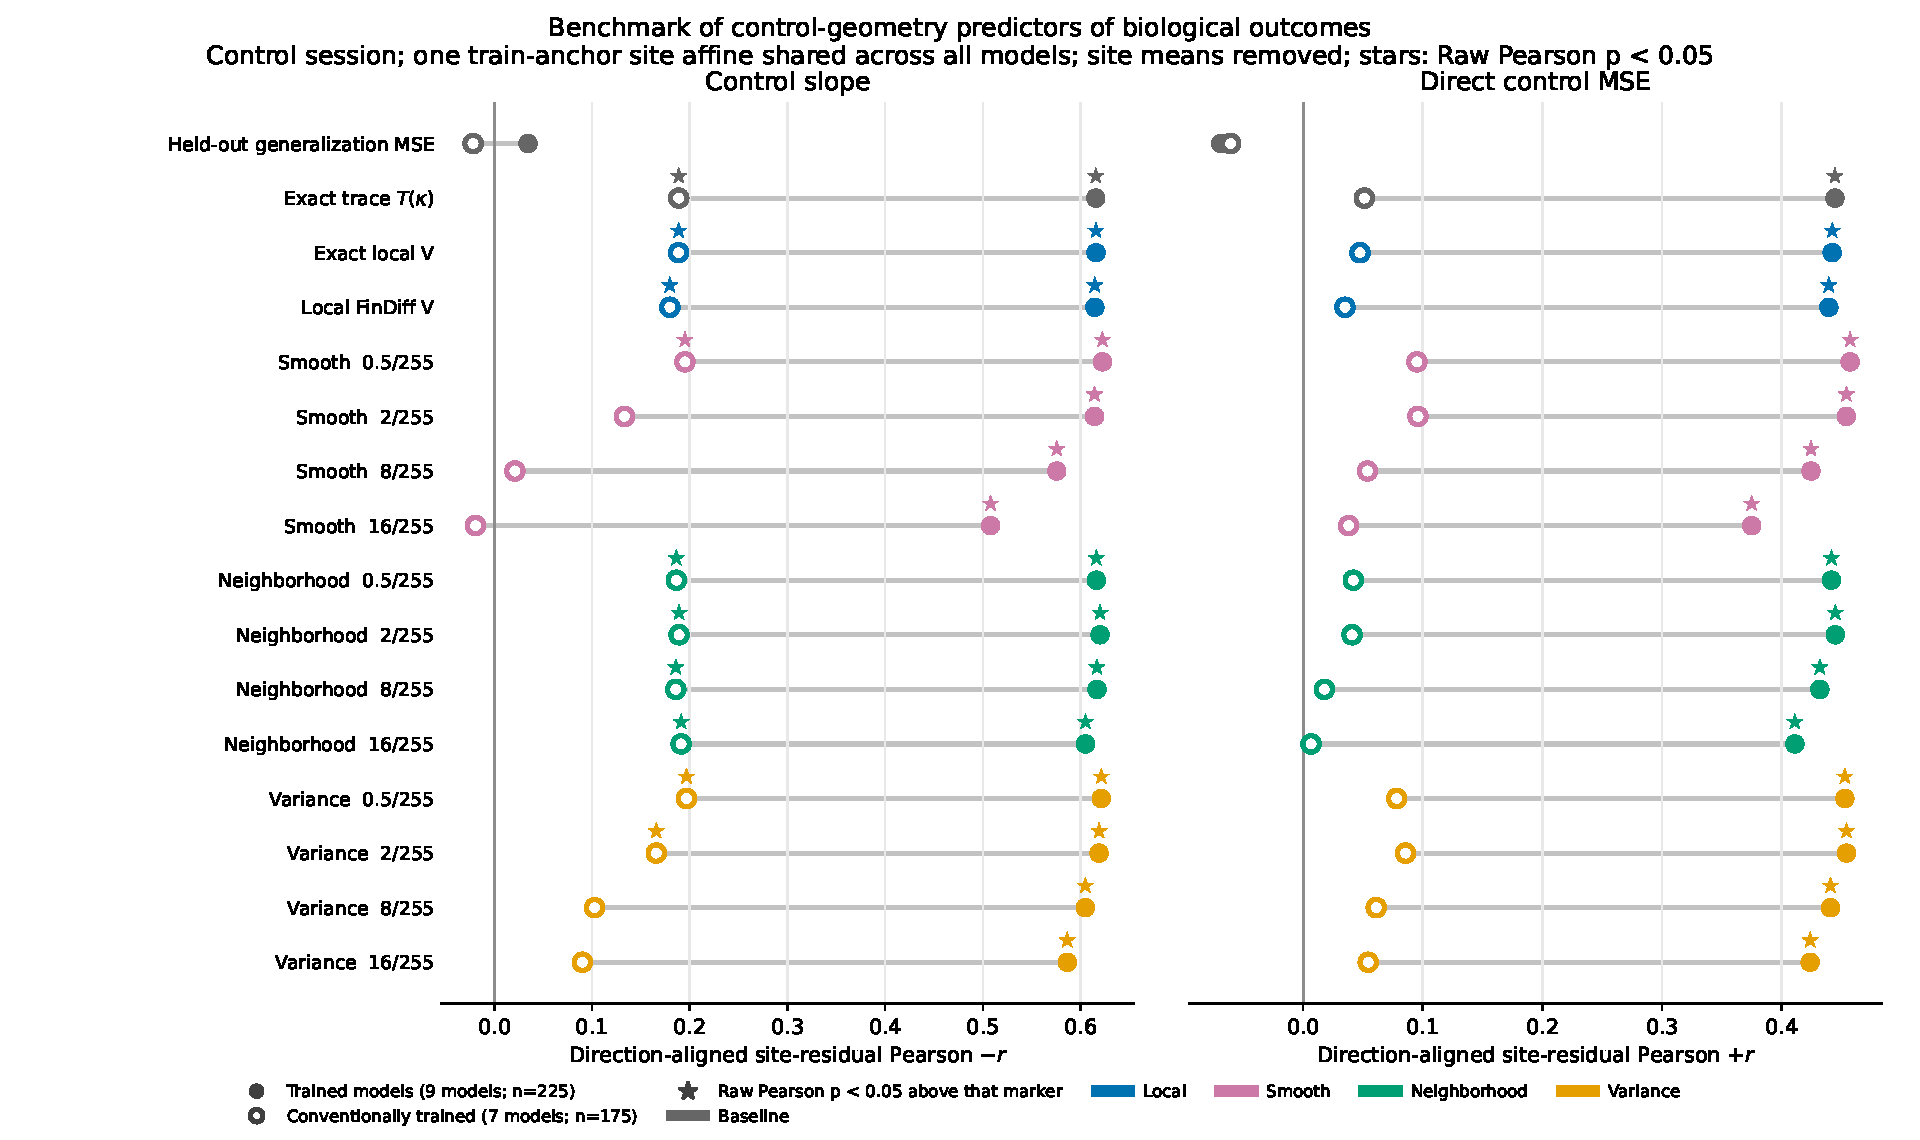
\includegraphics[width=\linewidth]{figures/nonlinear_control_biological_validation.pdf}
  \caption{\textcolor{red}{\textbf{Nonlinear gradient geometry predicts biological control across encoding models.}
  Each marker is a site-residual Pearson association between a candidate
  control-error predictor and biological control slope (left, sign reversed so
  larger means better error prediction) or direct control MSE (right).  Filled
  markers use the nine trained models ($n=225$ site--model pairs); open markers
  retain seven conventionally trained models ($n=175$).  Held-out natural-image
  error carries little model-order information in the nine-model comparison,
  whereas the exact trace, local $V_\phi$, and finite-neighborhood diagnostics
  recover substantial ordering.  Stars denote the figure's exploratory raw
  Pearson threshold; dependence across models and sites requires the qualified
  interpretation in the text.}}
  \label{fig:nonlinear-biological-validation}
\end{figure}
\endgroup

\subsection{Summary of the Cause}
\label{sec:diagnostics}

The preceding results separate three ingredients that jointly determine whether good prediction coexists with poor accentuation.
\todo{check this }
\paragraph{Input spectrum.}
Prediction measures weight error in the covariance geometry, $(\bhat-\bstar)^\top\Sigma(\bhat-\bstar)$, whereas accentuation uses the Euclidean direction $\bhat$.
A broad or rapidly decaying spectrum therefore creates directions that are cheap for prediction but consequential for control.
\red{For isotropic data with direct pixel regression ($F=I_d$), these two geometries are proportional and this particular hiding mechanism is absent. A non-orthogonal feature map can nevertheless reintroduce a mismatch even when $\Sigma=I_d$.}
Natural images provide the opposite regime: their low-variance tail is dominated by high-spatial-frequency modes, so visually unnatural weight components can have little effect on held-out prediction.

\paragraph{Noisy targets and finite samples.}
An anisotropic spectrum creates vulnerable directions but does not by itself populate them.
Finite-sample regression of noisy responses injects estimation variance into the fitted coefficients, with the weakest data modes being the least constrained.
Ridge regularization suppresses this amplification but generally does not remove it uniformly, especially when its strength is selected to optimize generalization rather than accentuation.
The pixel-space deterministic equivalent above quantifies how $\sigma$, $n$, and the spectrum jointly determine the hidden Euclidean weight error.

\paragraph{Feature map.}
Feature regression adds a second mismatch: prediction depends on the induced feature covariance and realizable teacher, whereas pixel-space accentuation backpropagates through $F$ and consequently depends on additional Euclidean statistics such as $FF^\top$.
Hence feature maps with indistinguishable prediction summaries can have sharply different accentuation behavior, as formalized by the gauge family above.
This identifies feature geometry---not predictive accuracy alone---as a diagnostic target: among equally predictive models, the more vulnerable map is the one that sends weakly constrained feature directions to large or poorly teacher-aligned pixel gradients.





\section{Related works}
\paragraph{Predictive model and control of neurons}


\paragraph{Ridge regression and OOD evaluation}


\paragraph{Degeneracy in linear model}




\clearpage




\iffalse

However, most theory works examined the population loss or test loss, i.e. evaluating the estimated model on the population distribution. => this is very similar to the experimental set up where the encoding models are evaluated on the held out images, and indeed this test loss does not show differences among many models.

Here our contribution is to study this system especially for our neural control experiment: what if we use the estimated models to propose new inputs to drive the system to a target state, what will be the error of control? How would that compares to the classic test error?

\paragraph{Set up}
We isolate this issue in the simplest high-dimensional model where it can be studied exactly: ridge regression with covariates $\x\sim\mathcal{N}(0,\Sigma)$ and responses
\begin{equation}
    y = {\btrue}^{\top} \x + \sigma \epsilon .
\end{equation}
The estimator is
\begin{equation}
    \bhat = (X^\top X + n\lambda I)^{-1}X^\top y.
\end{equation}
The usual generalization error is
\begin{equation}
    E_{\mathrm{gen}} = \mathbb{E}_{X,\epsilon,\x}\bigl[(\bhat-\btrue)^\top \x\bigr]^2
    = \mathbb{E}_{X,\epsilon}(\bhat-\btrue)^\top\Sigma(\bhat-\btrue).
\end{equation}

By contrast, ignoring the seed image $\x_0=0$, then the accentuation path lies on the direction of the estimated weight, with a scaling coefficient, $\x=\alpha \bhat$ with $\alpha\sim p_\alpha$.
We idealized the control experiment as above and study the case where the experimenters choose the target levels such that the model predicted response has the same variance as the observed response variance over the natural distribution, namely
$$Var_{\alpha\sim p_\alpha}[\bhat^\top (\alpha \bhat)]=Var_{\x\sim\mathcal{N}(0,\Sigma)}[\btrue \x]$$
under such case we have $Var[\alpha]=\frac{{\bstar}^{\top}\Sigma\bstar}{({\bhat}^{\top}\bhat)^{2}}$

Thus, an accentuation evaluation asks what happens when the fitted direction is used as the test path instead of the training distribution $\mathcal{N}(0,\Sigma)$.
% by asking if the experimenter with the fitted model will accentuate a sample, to reach the same dynamic range as the training


If a user moves along $\bhat$ but the target response should move along $\btrue$, the error is controlled by the scalar alignment ratio
\begin{equation}
    R=\frac{\bhat^\top\btrue}{\bhat^\top\bhat},
    \qquad
    \Eacc = {\btrue}^{\top}\Sigma\btrue \cdot \mathbb{E}\left[(1-R)^2\right].
\end{equation}
This quantity is not a reweighted version of $E_{\mathrm{gen}}$: it is sensitive to the direction and norm of $\bhat$, and it can be dominated by modes that contribute little to average test error.

This paper develops a random matrix theory (RMT) account of this dissociation. In the proportional limit $n,d\to\infty$ with $d/n\to\gamma$, we derive a deterministic equivalent for the per-principal-component coefficient error. The formula yields a closed-form decomposition of $E_{\mathrm{gen}}$ and an analytic prediction for the mean accentuation alignment.
% It also exposes the regime where leading-order RMT is insufficient: when the mean alignment is near one, $\operatorname{Var}(R)$ rather than $(1-\mathbb{E}R)^2$ controls $\Eacc$.

\fi 








\begin{figure}
    \centering
    % \includegraphics[width=0.5\linewidth]{}
    % \caption{\textbf{Linear theory of accentuation in visual neural models}. (A) Schematic of the accentuation phenomenon. A true neural weight w* and a model weight w share the same predictions on natural images (blue ellipse, high-variance axes), but diverge along the low-variance axis. During closed-loop accentuation, gradient steps along w push stimuli off the natural image manifold in the direction of low-variance eigenmodes, generating images that drive w strongly but fail to activate w*. (B) Natural image eigenspectrum and eigenmode gallery (van Hateren). The singular value spectrum decays steeply, spanning orders of magnitude. Top eigenmodes (high variance, k=0,1,4…) capture global luminance and low-spatial-frequency structure; bottom eigenmodes (k=−1,−4,−16…) encode high-frequency, noise-like textures invisible in natural statistics. (C) Eigenmode visualizations. Five high-variance (top row) and five low-variance (bottom row) eigenmodes shown as 100×100 images with their singular values. High-variance modes are smooth and spatially structured; low-variance modes are high-frequency and less structured. (D) Weight perturbation along low-variance modes has negligible effect on in-distribution prediction. Starting from a circle-mask ground truth w*, adding a large perturbation (α=1000) along the bottom eigenspace yields a visually very different weight, yet predictions on 1000 natural images are nearly identical (R²=1−4.42×10⁻³). (E) Diverse generation with similar prediction: accentuation experiment. Starting from a seed natural image, gradient accentuation using w₁ (w* with perturbation in mid-low eigenspace, α=1) produces images that preserve natural appearance while genuinely increasing f*(x). Accentuation using w₂ (w* with perturbation in bottom eigenspace, α=100) produces structurally altered, adversarial-like images that drive f₂ to target levels but leave f(x) near baseline — demonstrating failure of control. (F) Asymmetry of generation and evaluation. Scatter plots confirm that while both w₁- and w₂-accentuated images are well-evaluated by f₁ (top), only w₁-accentuated images show correlated f* responses (bottom left). w₂-accentuated images decouple completely from f* (bottom right), exposing the accentuation failure mode, but even w2 model can appreciate the success of w₁-accentuated images. (G) OLS/Ridge regression from noisy data contribute to this pattern. Linear regression with natural image data fails to recover the ground truth circle mask accurately under OLS or Ridge regression, both introduce spurious high-frequency components (low-variance eigenmodes) into the estimated weight, recapitulating the w₂ scenario. (H) Summary. Natural image statistics concentrate variance in low-spatial-frequency modes, leaving high-frequency directions in the near-null space. Regression solutions (especially OLS) absorb spurious correlations along these low-variance modes. In closed-loop neural experiments, such models generate adversarial high-frequency stimuli that drive the model strongly but fail to control the true neural response.}
    \label{fig:placeholder}
\end{figure}










\section{Reproducibility Statement}

The theory assumptions, derivations, and deterministic equivalents are stated in the main text, with full derivations intended for the appendix. The accompanying validation repository contains the core RMT library, CPU and GPU Monte Carlo scripts, notebooks recreating the figures, and saved outputs for the experiments shown here. The experiments use synthetic Gaussian covariates with specified spectra and empirical natural-image covariance spectra; all random quantities are generated by the scripts.

\section{Ethics Statement}

This work is theoretical and uses synthetic simulations and natural-image covariance spectra for validation. It does not introduce a deployed model, collect human-subject data, or release a dataset with personal information. The main risk is interpretive: directional analyses can be misleading if treated as causal without appropriate assumptions. The paper therefore emphasizes the limits of average test error and the assumptions required for the proposed metric.

\bibliography{iclr2026/accentuation_rmt_iclr2026}
\bibliographystyle{iclr2026/iclr2026_conference}

\clearpage
\appendix
\tableofcontents{}
\input{theory_appendix.tex}
% \section{Derivation Sketch for the Per-PC Formula}

% The ridge estimator can be written as
% \begin{equation}
%     \bhat-\btrue
%     =
%     -\lambda(\widehat{\Sigma}+\lambda I)^{-1}\btrue
%     +
%     \sigma(\widehat{\Sigma}+\lambda I)^{-1}\frac{1}{n}X^\top\epsilon,
% \end{equation}
% where $\widehat{\Sigma}=X^\top X/n$. Taking the squared projection onto $\uhat_k$, averaging over noise, and applying deterministic equivalents for one- and two-resolvent quadratic forms yields the bias, finite-sample signal, and finite-sample noise terms in equation~\ref{eq:per_pc}. The identity
% \begin{equation}
%     \frac{d\kappa}{d\lambda}=\frac{n}{n-\df(\kappa)}
% \end{equation}
% turns the derivative form of the noise term into the effective-sample-size denominator $n-\df(\kappa)$.

\section{ICLR 2026 Formatting Notes}

This draft uses the official ICLR 2026 style files. The author guide states that submissions are double blind, initial main text is limited to 9 pages, references do not count toward the page limit, and appendices are unlimited but optional for reviewers. The guide also recommends reproducibility and ethics statements before the references.
\end{document}



Average test error is a coarse statistic. It measures how well a fitted predictor performs under the test distribution, but it does not say whether the fitted direction is reliable when the predictor is used as a coordinate for intervention, extrapolation, or ``accentuation.'' In many representation-learning and scientific settings, the learned direction itself becomes an object of analysis: one moves along it to amplify a factor, reads off its alignment with a biological or perceptual axis, or studies model behavior under directional perturbations. A predictor can therefore have acceptable average error while inducing a misleading direction.


Our contributions are:
\begin{itemize}
    \item We derive a three-term deterministic equivalent for the per-eigenmode ridge coefficient error under general population spectrum $\Sigma$ and arbitrary signal orientation $\btrue$.
    \item We use this formula to predict a directional accentuation error and to identify when accentuation error and ordinary generalization error cross as the noise level changes.
    \item We validate the theory across synthetic spectra and natural-image covariance spectra, including GPU Monte Carlo experiments up to $d=10{,}000$.
    \item We diagnose a second-order alignment-variance gap and give a delta-method correction showing why leading deterministic equivalents accurately predict $\mathbb{E}[R]$ but can underpredict $\mathbb{E}[(1-R)^2]$ in high-noise regimes.
\end{itemize}

\section{Related Work}

High-dimensional linear regression has been a central testbed for understanding bias, variance, interpolation, and regularization in modern machine learning \citep{dobriban2018high,hastie2022surprises,mei2022generalization}. Deterministic equivalents from random matrix theory provide sharp asymptotic predictions for ridge risk under anisotropic covariance and proportional scaling \citep{bai2010spectral,couillet2011random}. Our work uses this toolbox but shifts the target from scalar predictive risk to a directional error induced by using the learned coefficient vector as an intervention axis.

The problem is also related to representation analysis and feature visualization, where learned directions are used to generate or accentuate semantic factors \citep{olah2017feature,bau2017network}. In such settings, average predictive accuracy is not sufficient: one needs the learned direction to be geometrically aligned with the intended factor. The accentuation metric studied here is a minimal linear analogue of this directional reliability problem.

\section{Setup and Deterministic Equivalent}

Represent true weight on the covariance eigenbasis, let $\Sigma=\sum_{k=1}^{d}\lambda_k \uhat_k\uhat_k^\top$ and write $b_k=\uhat_k^\top\btrue$.

Define $\kappa=\kappa(\lambda)$ as the positive solution of the fixed-point equation
\begin{equation}
    \kappa-\lambda
    = \gamma\kappa \frac{1}{d}\sum_{j=1}^{d}\frac{\lambda_j}{\kappa+\lambda_j}.
    \label{eq:kappa}
\end{equation}
We also define
\begin{equation}
    \df(\kappa)=\sum_{j=1}^{d}\frac{\lambda_j^2}{(\lambda_j+\kappa)^2},
    \qquad
    C_{\mathrm{sig}}(\kappa)=\sum_{j=1}^{d}\frac{\lambda_j b_j^2}{(\lambda_j+\kappa)^2}.
\end{equation}

\begin{proposition}[Per-eigenmode ridge error]
Under the Gaussian design model above and in the proportional high-dimensional limit, the squared coefficient error along the $k$th population eigenvector satisfies the deterministic equivalent
\begin{align}
    \mathbb{E}\bigl[(\uhat_k^\top(\bhat-\btrue))^2\bigr]
    &\asymp
    \underbrace{\frac{\kappa^2}{(\lambda_k+\kappa)^2}b_k^2}_{\text{regularization bias}}
    +
    \underbrace{
    \frac{1}{n-\df(\kappa)}
    \frac{\lambda_k\kappa^2}{(\lambda_k+\kappa)^2}
    C_{\mathrm{sig}}(\kappa)}_{\text{finite-sample signal fluctuation}}
    \nonumber\\
    &\quad+
    \underbrace{
    \frac{\sigma^2}{n-\df(\kappa)}
    \frac{\lambda_k}{(\lambda_k+\kappa)^2}}_{\text{finite-sample noise amplification}} .
    \label{eq:per_pc}
\end{align}
\end{proposition}

The three terms in equation~\ref{eq:per_pc} have distinct geometric meanings. The first term is deterministic shrinkage of true signal along eigenmodes of $\Sigma$. The second is a finite-sample fluctuation of the signal component induced by the random training design. The third is noise amplification; it peaks around $\lambda_k\approx\kappa$ and grows as $\kappa$ becomes small. Ordinary test error is obtained by summing equation~\ref{eq:per_pc} with weights $\lambda_k$:
\begin{equation}
    E_{\mathrm{gen}}\asymp
    \sum_{k=1}^{d}\lambda_k\,
    \mathbb{E}\bigl[(\uhat_k^\top(\bhat-\btrue))^2\bigr].
\end{equation}

\section{Accentuation Error}

The accentuation metric depends on the ratio
\begin{equation}
    R=\frac{\bhat^\top\btrue}{\bhat^\top\bhat}.
\end{equation}
Using equation~\ref{eq:per_pc}, the deterministic equivalents for numerator and denominator are
\begin{align}
    N_{\det}
    &= \sum_{k=1}^{d}\frac{\lambda_k}{\lambda_k+\kappa}b_k^2,\\
    D_{\det}
    &= \sum_{k=1}^{d}\left(\frac{\lambda_k}{\lambda_k+\kappa}\right)^2b_k^2
    +
    \frac{\kappa^2 C_{\mathrm{sig}}+\sigma^2}{n-\df(\kappa)}
    \sum_{k=1}^{d}\frac{\lambda_k}{(\lambda_k+\kappa)^2}.
\end{align}
Thus $R_{\det}=N_{\det}/D_{\det}$, and the leading accentuation prediction is
\begin{equation}
    \Eacc^{(0)}
    =
    {\btrue}^{\top}\Sigma\btrue\,(1-R_{\det})^2.
    \label{eq:eacc0}
\end{equation}

Equation~\ref{eq:eacc0} makes the dissociation from ordinary generalization explicit. $E_{\mathrm{gen}}$ weights per-mode error by the data variance $\lambda_k$, while accentuation depends on the ratio of two global quadratic forms in $\bhat$. As a result, the same ridge penalty can reduce average prediction error while producing a fitted direction whose extrapolation scale is biased.

\section{Experiments}

We evaluate the deterministic equivalents on three spectra: isotropic covariance, power-law covariance, and empirical covariance from van Hateren natural-image patches. Monte Carlo estimates are computed by repeatedly sampling $X$ and response noise, fitting ridge regression, and comparing the fitted coefficient vector to the ground-truth coefficient vector. For large dimensions we use the kernel form of ridge regression and GPU Monte Carlo.

\begin{figure}[t]
    \centering
    
\includegraphics[width=\textwidth]{../figures/nb_small_d_per_pc.png}
    \caption{Per-eigenmode coefficient error. The three-term deterministic equivalent tracks Monte Carlo estimates across isotropic, power-law, and natural-image spectra, including the shape of the error across population PCs.}
    \label{fig:per_pc}
\end{figure}

Figure~\ref{fig:per_pc} validates equation~\ref{eq:per_pc} at small dimension, where per-PC Monte Carlo estimates are directly observable. The theory captures not only total error but also the anisotropic distribution of coefficient error across eigendirections.

\begin{figure}[t]
    \centering
    
\includegraphics[width=\textwidth]{../figures/nb_large_d.png}
    \caption{Large-dimensional validation. GPU simulations agree with the deterministic equivalent for power-law spectra and natural-image covariance spectra up to $d=10{,}000$.}
    \label{fig:large_d}
\end{figure}

Figure~\ref{fig:large_d} confirms that the formulas remain accurate in the high-dimensional regime where the asymptotic theory is intended to apply. On power-law and natural-image spectra, total generalization error agrees with Monte Carlo to within the small gaps reported in the validation code.

\begin{figure}[t]
    \centering
    
\includegraphics[width=\textwidth]{../figures/sigma_sweep_fixed_accentuation.png}
    \caption{Noise sweep. The deterministic equivalent tracks ordinary generalization error and the mean accentuation alignment across noise levels. Correctly accounting for finite-sample signal variance in $D_{\det}$ is essential for the alignment prediction.}
    \label{fig:sigma}
\end{figure}

Figure~\ref{fig:sigma} shows a sweep over response noise. The leading RMT prediction matches average generalization error across the full range, and it accurately predicts the mean alignment ratio $R$. This experiment also identifies a practical failure mode in incomplete formulas: replacing $\mathbb{E}[\bhat^\top\bhat]$ by a squared mean omits the finite-sample signal term and produces a biased alignment estimate.

\begin{figure}[t]
    \centering
    
\includegraphics[width=.82\textwidth]{../figures/gen_vs_acc_optimal_lambda_vh.png}
    \caption{Generalization--accentuation crossing on van Hateren spectra. With $\lambda$ chosen to minimize predicted generalization error at each $\sigma$, the theory predicts the noise level at which ordinary test error overtakes accentuation error.}
    \label{fig:crossing}
\end{figure}

Figure~\ref{fig:crossing} illustrates the central qualitative prediction. At low noise, directional accentuation error can dominate because regularization biases the learned direction. At high noise, ordinary prediction error dominates because noise contaminates the coefficient estimate. The crossing point gives a concise operating-regime summary.

\section{Second-Order Gap: Variance of the Alignment Ratio}

The leading accentuation formula uses
\begin{equation}
    \mathbb{E}[(1-R)^2]\approx (1-R_{\det})^2.
\end{equation}
This is accurate when the bias term dominates. However,
\begin{equation}
    \mathbb{E}[(1-R)^2]=(1-\mathbb{E}R)^2+\operatorname{Var}(R),
\end{equation}
so a leading deterministic equivalent for $\mathbb{E}R$ is insufficient when $R$ concentrates near one.

Let $N=\bhat^\top\btrue$, $D=\bhat^\top\bhat$, and $R_{\det}=N_{\det}/D_{\det}$. A delta-method expansion gives
\begin{equation}
    \operatorname{Var}(R)\asymp
    \frac{\operatorname{Var}(N-R_{\det}D)}{D_{\det}^{2}}.
\end{equation}
Writing $\bhat=g+h$ with deterministic signal component $g\approx(\Sigma+\kappa I)^{-1}\Sigma\btrue$ and noise component $h$, the noise-driven contribution is
\begin{align}
    \operatorname{Var}(R)
    &\approx
    \frac{1}{D_{\det}^{2}}
    \left[
    \frac{\sigma^2}{n}
    \sum_k
    \frac{\lambda_k b_k^2}{(\lambda_k+\kappa)^2}
    \left(1-\frac{2R_{\det}\lambda_k}{\lambda_k+\kappa}\right)^2
    +
    \frac{2R_{\det}^2\sigma^4}{n^2}
    \sum_k
    \frac{\lambda_k^2}{(\lambda_k+\kappa)^4}
    \right].
    \label{eq:varr}
\end{align}
Equation~\ref{eq:varr} captures the correct order and growth with $\sigma$, but a full correction also requires fluctuations from the random design $X$ itself. This explains why the mean alignment in Figure~\ref{fig:sigma} is accurate while the full second moment can be underestimated in high-noise regimes.

\begin{figure}[t]
    \centering
    
\includegraphics[width=.82\textwidth]{../figures/var_R_theory_vs_mc.png}
    \caption{Variance correction for the alignment ratio. The missing $\operatorname{Var}(R)$ term is negligible when alignment bias is large, but can dominate $\Eacc$ when $R$ is close to one.}
    \label{fig:varr}
\end{figure}

\section{Discussion}

The analysis suggests a simple lesson: evaluating a model by average prediction error can miss failures that appear when the model is used directionally. In ridge regression, the problem is already visible and exactly characterizable. The learned vector is pulled by regularization, finite-sample covariance fluctuations, and noise amplification in ways that affect average prediction and directional accentuation differently.

This setting is intentionally minimal. It does not claim that nonlinear representation accentuation reduces to ridge regression. Instead, it provides a solvable baseline for a broader phenomenon: when learned directions are used as coordinates for intervention, their geometry matters independently of scalar predictive risk. The RMT formulas identify which parts of the data spectrum and signal orientation control this geometry.

The main technical limitation is second-order fluctuation theory. Leading deterministic equivalents are enough for per-PC error, ordinary generalization, and mean alignment. They are not enough for the full accentuation second moment in regimes where $\operatorname{Var}(R)$ dominates. A complete treatment should combine deterministic equivalents with central limit theorems for quadratic functionals of anisotropic Wishart matrices.
